\documentclass[11pt]{article}
\usepackage{ucs}
\usepackage{graphicx}
\usepackage[utf8x]{inputenc} 
\usepackage[russian]{babel}  
\usepackage{geometry}

\geometry{left=2cm}
\geometry{right=1.5cm}
\geometry{top=2cm}
\geometry{bottom=2cm} 


\title{ Техническая книга, ФМЛ №30, команда ПСИ}

\begin{document}
	\maketitle
	\tableofcontents{}
	\newpage
	
	\section{Состав команды}
		\begin{table}[h]
			\begin{tabular}{|l|l|l|l|}
				\hline
				\textit{ФИО}         & Год рождения & Место учебы   & Роль в команде                      \\ \hline
				Жадковский Александр &  1998        & ФМЛ №30       & Капитан команды                     \\ \hline
				Лутошкин Роман       &  1998        & Гимназия №642 & Ответственный за техническую книгу, \\
				                     &              &               & оператор № 1                        \\ \hline
				Ильясов Александр    &  1999        & ФМЛ №30       & Оператор №2                         \\ \hline
				Поникаровский Антон  & 1998         & ФМЛ №30       & Запасной оператор                   \\ \hline
			\end{tabular}
		\end{table}
	\section{Описание робота}
		\subsection{Конструкция}
			\begin{itemize}
				\item Робот должен быть небольшим и мобильным
				\item Конструкция должна быть наиболее простой с максимально легким доступом ко всем узлам конструкции
				\item Робот должен обладать механизмом подъема, способным подниматься на высоту 120 см и выше
				\item По возможности робот должен обладать специальным приспособлением для зацепки корзин и их перемещения
			\end{itemize}
		\subsection{Стратегия}
			Период выступления делится на 2(3) периода: автономный период и основное время, которое состоит из первых 1.5 минут и последних 30 секунд.
			В автономном периоде робот должен:
			\begin{itemize}
				\item В зависимости от расположения, съехать с пандуса или выехать вперед
				\item Сориентироваться согласно ИК-датчику и сбить подпорку корзины
				\item Захватить максимально возможное кол-во шариков(Но не более 5-ти)
			\end{itemize}
			После автономного периода следует управляемый двухминутный период в котором необходимо:
			\begin{itemize}
				\item Выгрузить захваченые в автономном периоде шарики в центр. корзину
				\item Захватить новые шарики 
				\item Повторять такую процедуру до окончания времени
				\item В конце вернуться на зону парковки
			\end{itemize}
		
	\section{Основная часть}
	
	\subsection{16.09.14}
	
	\begin{enumerate}
		\item Дата собрания : 16.09.14
		\item Цель:
		\begin{itemize}
			\item Собрать основу робота, а именно колесную базу
			\item Написать простейшую программу для управления роботом
		\end{itemize}			
		\item Реализация :
		\begin{itemize}
			\item Была собрана квадратная конструкция(Рис. 1)
			\item Написана программа для передвижения
		\end{itemize}
		\item Результаты
		\begin{itemize}
			\item Собран четырехколесный робот, способный передвигаться по четырем направлениям
			\item Робот управляется с помощью геймпада
		\end{itemize}
		Получившаяся конструкция:
		\begin{figure} [h]
			\centering
			\begin{minipage}{0.3\linewidth}
				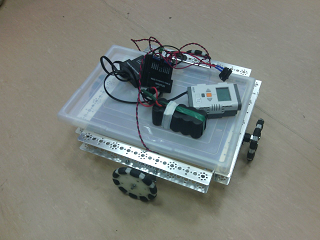
\includegraphics[width=35mm,height=35mm]{Days/16.09.14/1_1_robot.png}\\ Рисунок 1
			\end{minipage}
			\begin{minipage}{0.3\linewidth}
				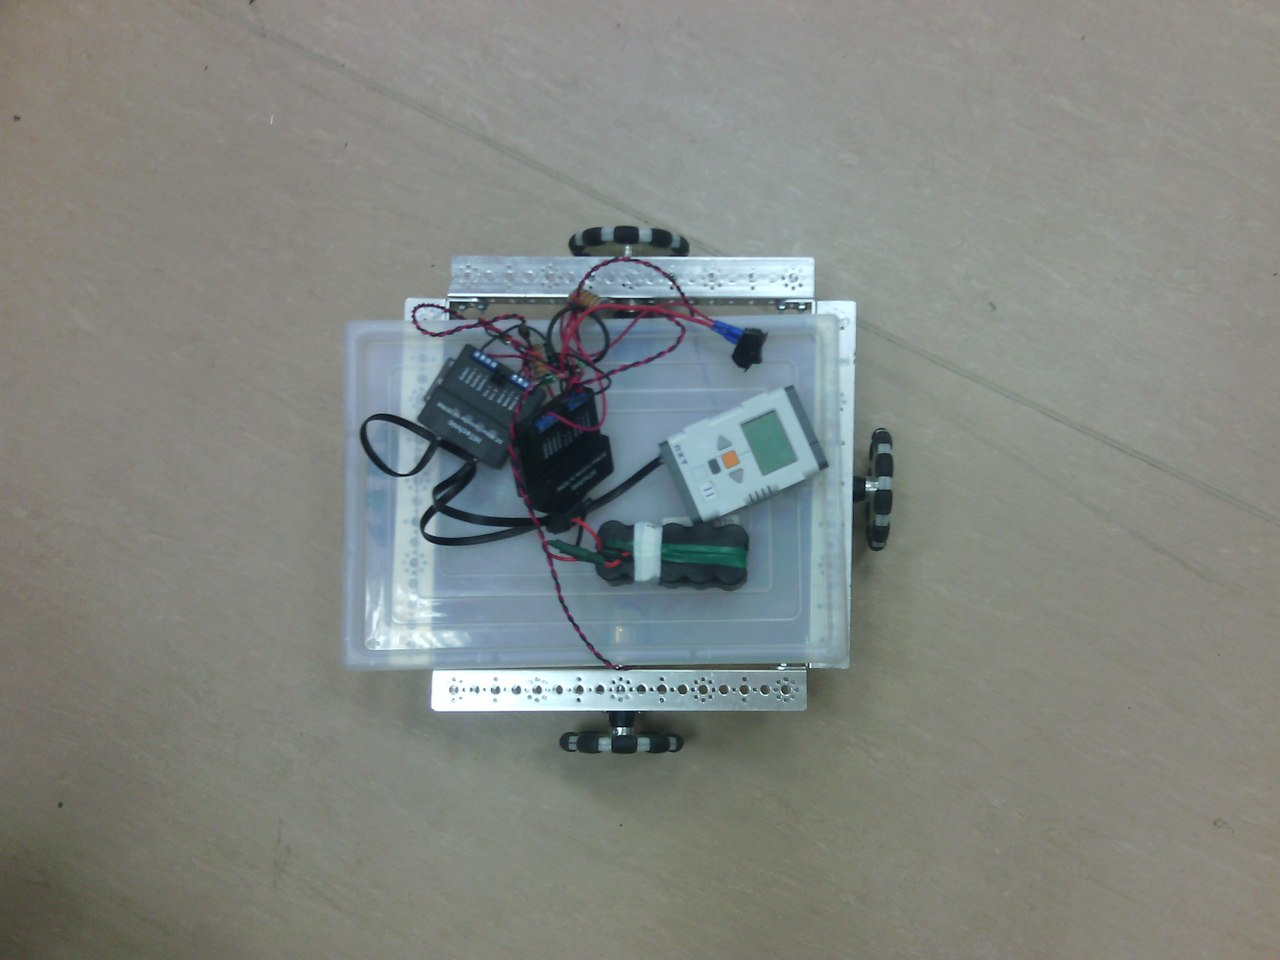
\includegraphics[width=35mm,height=35mm]{Days/16.09.14/1_2_robot}\\ Рисунок 2
			\end{minipage}
		\end{figure}
	\end{enumerate}
	
	\subsection{3.10.14}
	
\begin{enumerate}
		\item Дата собрания 3.10.14
		\item Цель:
		\begin{itemize}
			\item Укрепить конструкцию робота
			\item Разнести колеса по углам конструкции для увеличения площади колесной базы
			\item Закрепить основные узлы управления робота на конструкции с максимально легким доступом к ним
			\item Оптимизировать программу, перенести управление передвижением робота с кнопок на джойстик
		\end{itemize}
		\item Результаты:
		\begin{itemize}
			\item Конструкция робота была укреплена, центр тяжести снижен 
			\item Двигатели были закреплены по углам конструкции, одновременно закрепляя ее
			\item На осях был закреплен второй ряд колес определенным образом для лучшего управления(Рисунок 2,3)
		\end{itemize}
		\begin{figure} [h]
			\centering
			\begin{minipage}{0.3\linewidth}
				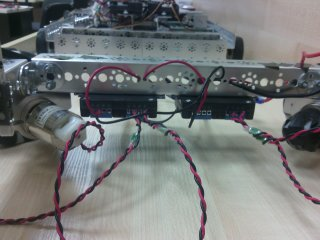
\includegraphics[width=35mm,height=35mm]{Days/3.10.14/3_1_robot}\\ Рисунок 3
			\end{minipage}
			\begin{minipage}{0.3\linewidth}
				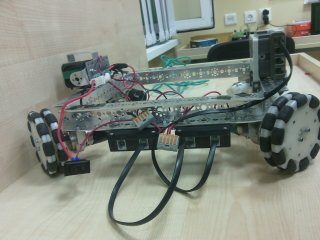
\includegraphics[width=35mm,height=35mm]{Days/3.10.14/3_2_robot}\\ Рисунок 4
			\end{minipage}
			\begin{minipage}{0.3\linewidth}
				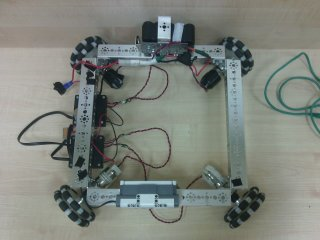
\includegraphics[width=35mm,height=35mm]{Days/3.10.14/3_3_robot}\\ Рисунок 5
			\end{minipage}
		\end{figure}
		\item Идеи и планы для следующего занятия:
		\begin{itemize}
			\item Начать строить механизм захвата и подъема шариков. В качесте механизма подъема можно использовать ножничный подъемник, механизм захвата еще обдумывается
		\end{itemize}
	\end{enumerate}
	\fillpage
\newpage
	
	\subsection{13.10.14}
	
	\begin{enumerate}
		\item Цель:
		\begin{itemize}
			\item Реализовать ножничный подъемник, механизм, приводящий его в движение и закрепление на кострукции робота
			\item Написать программу для управления захватом с отдельного геймпада
		\end{itemize}
		\item Результаты:
		\begin{itemize}
			\item Робот был частично разобран из-за недостатка деталей, была собрана примерная схема механизма передвижения подъемника(Рисунок 6)
			\item Написать и отладить программу не получилось, опять же из-за отсутствия деталей
			\item При тестировании барабана для намотки лески обнаружился очень сильный изгиб конструкции во время вращения барабана. Возможно, проблема в неоткалиброванном барабане или осях моторов, находящихся на разных уровнях. Попытаемся исправить это на следующем занятии.
		\end{itemize}
		\item Идеи:
		\begin{itemize}
			\item Заменить текущие рейки в подъемнике на алюминиевые профили для удобства установки, увеличения длины составляющих подъемника и уменьшения веса конструкции
			\item Отказаться от омниколес, поставить 4 обычных колеса
		\end{itemize}
		\item Рисунки:
		\begin{figure} [h]
			\centering
			\begin{minipage}{0.3\linewidth}
				\includegraphics[width=40mm,height=25mm]{Days/13.10.14/5_1_robot}\\ Рисунок 6
			\end{minipage}
			\begin{minipage}{0.3\linewidth}
				\includegraphics[width=40mm,height=25mm]{Days/13.10.14/5_2_robot}\\ Рисунок 7
			\end{minipage}
		\end{figure}
	\end{enumerate}
	\clearpage

	
	\subsection{15.10.14}
	
	\begin{enumerate}
	\item Дата собрания: 15.10.14
	\item Цель:
		\begin{itemize}
		\item Заменить омни-колеса на обычные
		\item Начать готовить профили для подъемника
		\item Решить проблему с барабаном
		\end{itemize}
	\item Результаты:
		\begin{itemize}
		\item Было установлено два колеса, оба ведущие. Так как теперь они установлены не в углах конструкции уменьшилась площадь опорной поверхности $\Rightarrow$ уменьшилась стабильность робота.
		\item Профили были распилены на отдельные части определенного размера и пропилены отверстия для креплений
		\item Проблема не была решена, вся конструкция ходит туда-сюда по-прежнему. Было решено оставить этот элемент в покое на данный момент времени и заняться колесной базой.
		\end{itemize}
	\item Идеи и планы:
		\begin{itemize}
		\item Установить оставшиеся колеса и испытать робота на поле
		\item Начать строить подъемник
		\end{itemize}
		\begin{figure} [h]
			\centering
			\begin{minipage}{0.3\linewidth}
				\includegraphics[width=35mm,height=35mm]{Days/15.10.14/8_1_robot}\\ Рисунок 8
			\end{minipage}
		\end{figure}
	\end{enumerate}
\fillpage
\newpage


	
	\subsection{17.10.14}
	
	\begin{enumerate}
	\item Дата собрания: 17.10.14
	\item Цель:
		\begin{itemize}
		\item Установить оставшиеся колеса, проверить подвижность робота(способность разворачиваться, заезжать на пандус и спускаться с него)
		\item Придумать(по возможности установить) конструкцию подъемника
		\end{itemize}
	\item Результаты:
		\begin{itemize}
		\item Проведя несколько пробных заездов с уже собранной конструкцией выяснилось, что робт имеет недостаточное сцепление с полем. Было решено заменить текущую колесную базу на трехколесную.
		\item Подходящих креплений для установки подъемника не нашлось. Крепления должны прочно, без люфтов, скреплять балочные элементы подъемника, при этом не создавая большого трения между ними.
		\item Для уменьшения люфтов и трения в основании конструкции были установлены выдвижные рейки(Рисунки 8, 9)
		\end{itemize}
	\item Идеи и планы:
		\begin{itemize}
		\item Установть вместо двух опорных омни-колес одно
		\item Появилась идея использовать в качестве креплений для подъемника мебельные стяжки.
		\end{itemize}
	\begin{figure} [h]
			\centering
			\begin{minipage}{0.3\linewidth}
				\includegraphics[width=35mm,height=35mm]{/!my_data/projects/pml30-psi_team/Days/17.10.14/7_1_robot}\\ Рисунок 8
			\end{minipage}
			\begin{minipage}{0.3\linewidth}
				\includegraphics[width=35mm,height=35mm]{/!my_data/projects/pml30-psi_team/Days/17.10.14/7_2_robot}\\ Рисунок 9
			\end{minipage}
			\begin{minipage}{0.3\linewidth}
				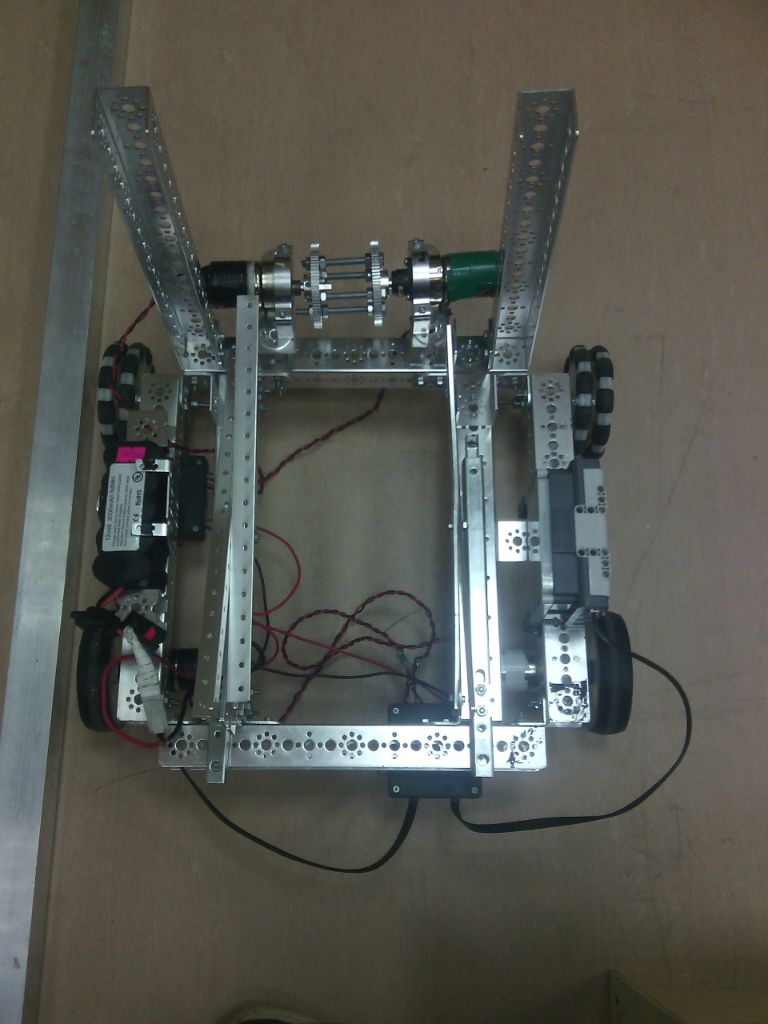
\includegraphics[width=35mm,height=35mm]{/!my_data/projects/pml30-psi_team/Days/17.10.14/7_3_robot}\\ Рисунок 10
			\end{minipage}		
	\end{figure}
	\end{enumerate}
\newpage

	\subsection{24.10.14}
	
	\begin{enumerate}
		\item Дата собрания: 24.10.14
		\item Цель:
		\begin{itemize}
			\item Установить одно опорное колесо вместо двух
			\item Попробовать мебельные стяжки в качестве креплений балочных элементов подъемника
			\item Проверить подвижность робота
		\end{itemize}			
		\item Результаты:
		\begin{itemize}
			\item Приводные колеса робота были отодвинуты назад примерно на 5см, так как робот очень часто вставал на задние колеса и переворачивался
			\item Стяжки хорошо проявили себя в качестве креплений: они не создают почти никакого трения, при этом сохраняя стабильность конструкции
			\item Робот оказался довольно подвижным, забирается на пандус, разворачивается на нем и спускается без проблем
			\item Программа была написана для максимально легкого управления
		\end{itemize}
		\item Идеи и планы:
		\begin{itemize}
			\item Оставить колесную базу в покое и начать строить только подъемник
		\end{itemize}
		\begin{figure} [h]
			\centering
			\begin{minipage}{0.3\linewidth}
				\includegraphics[width=35mm,height=35mm]{/!my_data/projects/pml30-psi_team/Days/24.10.14/9_1_robot}\\ Рисунок 11
			\end{minipage}
			\begin{minipage}{0.3\linewidth}
				\includegraphics[width=35mm,height=35mm]{/!my_data/projects/pml30-psi_team/Days/24.10.14/10_2_robot}\\ Рисунок 12
			\end{minipage}
			\begin{minipage}{0.3\linewidth}
				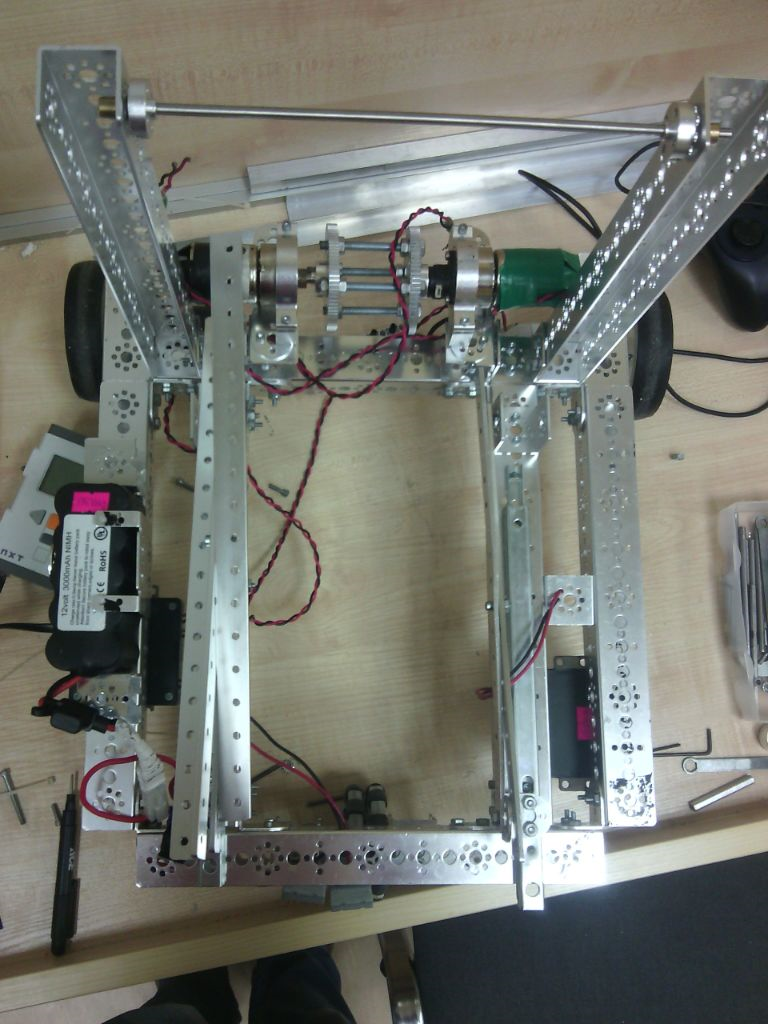
\includegraphics[width=35mm,height=35mm]{/!my_data/projects/pml30-psi_team/Days/24.10.14/9_4_robot}\\ Рисунок 13
			\end{minipage}
		\end{figure}
	\end{enumerate}
\newpage	
	
	\subsection{5.11.14}
	
	\begin{enumerate}
		\item Дата собрания: 5.11.14
		\item Цель:
		\begin{itemize}
			\item Полностью собрать подъемник и испытать его
			\item Написать программу для управления им
		\end{itemize}			
		\item Реализация:
		\begin{itemize}
			\item Подъемник был собран, под стяжки пришлось расширить уже просверленые отверстия
			\item Механизм передвижения подъемника был переделан на более простой.
		\end{itemize}
		\item Результаты:
		\begin{itemize}
			\item Шестеренки при подъеме конструкции соскальзывали из-за слишком большого усилия, оси слышком сильно выгибались по той же причине.
		\end{itemize}
		\item Идеи и планы:
		\begin{itemize}
			\item Поставить меньшее передаточное отношение
			\item Установить более прочные оси
		\end{itemize}
		\begin{figure} [h]
			\centering
			\begin{minipage}{0.3\linewidth}
				\includegraphics[width=35mm,height=35mm]{Days/5.11.14/10_1_robot}\\ Рисунок 14
			\end{minipage}
			\begin{minipage}{0.3\linewidth}
				\includegraphics[width=35mm,height=35mm]{Days/5.11.14/10_3_robot}\\ Рисунок 15
			\end{minipage}
		\end{figure}
	\end{enumerate}
\newpage	
\end{document}
